% Opcje klasy 'iithesis' opisane sa w komentarzach w pliku klasy. Za ich pomoca
% ustawia sie przede wszystkim jezyk i rodzaj (lic/inz/mgr) pracy, oraz czy na
% drugiej stronie pracy ma byc skladany wzor oswiadczenia o autorskim wykonaniu.
\documentclass[declaration,shortabstract]{iithesis}

\usepackage[utf8]{inputenc}
\usepackage{graphicx}

%%%%% DANE DO STRONY TYTUŁOWEJ
% Niezaleznie od jezyka pracy wybranego w opcjach klasy, tytul i streszczenie
% pracy nalezy podac zarowno w jezyku polskim, jak i angielskim.
% Pamietaj o madrym (zgodnym z logicznym rozbiorem zdania oraz estetyka) recznym
% zlamaniu wierszy w temacie pracy, zwlaszcza tego w jezyku pracy. Uzyj do tego
% polecenia \fmlinebreak.
\polishtitle    {Analiza statyczna języka Ruby}
\englishtitle   {Static analysis for Ruby language}
\polishabstract {\ldots}
\englishabstract{\ldots}
% w pracach wielu autorow nazwiska mozna oddzielic poleceniem \and
\author         {Rafał Łasocha}
% w przypadku kilku promotorow, lub koniecznosci podania ich afiliacji, linie
% w ponizszym poleceniu mozna zlamac poleceniem \fmlinebreak
\advisor        {prof. Witold Charatonik}
%\date          {}                     % Data zlozenia pracy
% Dane do oswiadczenia o autorskim wykonaniu
%\transcriptnum {}                     % Numer indeksu
%\advisorgen    {dr. Jana Kowalskiego} % Nazwisko promotora w dopelniaczu
%%%%%

%%%%% WLASNE DODATKOWE PAKIETY
%
%\usepackage{graphicx,listings,amsmath,amssymb,amsthm,amsfonts,tikz}
%
%%%%% WŁASNE DEFINICJE I POLECENIA
%
%\theoremstyle{definition} \newtheorem{definition}{Definition}[chapter]
%\theoremstyle{remark} \newtheorem{remark}[definition]{Observation}
%\theoremstyle{plain} \newtheorem{theorem}[definition]{Theorem}
%\theoremstyle{plain} \newtheorem{lemma}[definition]{Lemma}
%\renewcommand \qedsymbol {\ensuremath{\square}}
% ...
%%%%%

\begin{document}

\chapter{Wprowadzenie}

Współcześnie powstaje wiele narzędzi ułatwiających i przyśpieszających pracę programistów.
W szczególności istnieją zintegrowane środowiska programistyczne (IDE), które próbują dostarczyć jak najwięcej takich narzędzi w jednym spójnym środowisku. Wśród najbardziej podstawowych funkcjonalności takich środowisk można znaleźć m. in.:

\begin{itemize}
\item skok do definicji (stałej, funkcji lub zmiennej)
\item informacja o typie zmiennej
\item autouzupełnianie pełnej nazwy aktualnie pisanej stałej, zmiennej lub nazwy funkcji
\end{itemize}

Niniejsza praca przedstawia jak można wykorzystać analizę statyczną plików źródłowych, aby dostarczyć powyższe funkcjonalności w języku Ruby, który z racji swojej dynamicznej natury stawia pewne problemy nie występujące w językach statycznie typowanych.

\section{Założenia i cele}

\subsection{Utrudnienia w językach słabo typowanych}

Zintegrowane środowiska nie są niczym nowym i są popularne wśród programistów od wielu lat.
Jednakże, trudność implementacji narzędzi bazujących na analizie kodu źródłowego zależy od niektórych cech języków programowania.
W językach silnie typowanych jest to znacznie prostsze, ponieważ gdy wiemy już jakiego typu jest zmienna -- lista dostępnych nazw funkcji jest łatwa do obliczenia (autouzupełnianie, skok do definicji). 
Podobnie, języki silnie typowane często mają \textit{static dispatch}, więc w momencie kompilacji wiemy gdzie jest kod źródłowy, który zostanie użyty w danym wywołaniu funkcji (skok do definicji).
Oczywiście, w każdym języku możemy używać konstrukcji, które to zadanie znacznie utrudniają (np. w C, wywołanie funkcji która jest przechowana we wskaźniku), ale nie używa się ich zbyt często.
W językach dynamicznie typowanych (takich jak Ruby, Python), gdzie język nie dostarcza kompilatora, który dostarczałby informacji o kodzie źródłowym, informacje te musimy sobie znaleźć sami.

\subsection{Utrudnienia w Ruby}

W języku Ruby, o którym jest ta praca, statyczne wywnioskowanie typu wyrażenia jest szczególnie ciężkie z dwóch powodów:
\begin{itemize}
\item wiele różnych dostępnych konstrukcji języka, takich jak wielokrotne dziedziczenie, klasy singletonowe, \textit{prepend} (przypis: nie wiem jak ten mechanizm się nazywa w nomenklaturze języków programowania) sprawia że zbudowanie hierarchii klas i poruszanie się po niej jest niełatwe
\item społeczność rubiego jest przyzwyczajona do korzystania z metaprogramowania w bibliotekach i projektach, a dynamicznie generowane (w czasie uruchomienia programu) nazwy zmiennych, metod oraz klas sprawiają że efektywna statyczna analiza tych fragmentów kodu jest niemożliwa
\end{itemize}

\subsection{Aktualny stan}

Do tworzenia oprogramowania w Ruby, programiści najczęściej wykorzystują Rubymine IDE lub edytory tekstu wspierane wtyczkami, takie jak Vim, Emacs czy Atom (przypis: strzał na razie, ale nic istotnego to nie zmieni).
Rubymine dostarcza funkcjonalności wspomnianych we wstępie, jednak jest to narzędzie płatne i zamknięte.
Edytory tekstu same w sobie nie posiadają tych funkcjonalności, ale istnieją wtyczki, które w jakiejś części te funkcjonalności dostarczają. Jak to bywa z analizą statyczną, efektywność tych narzędzi to pewne spektrum, jedne narzędzia dostarczają lepsze autouzupełnianie, a inne gorsze. Nie jest to binarne i jakość tych funkcjonalności ma duże znaczenie dla programisty.
Najpopularniejsze wtyczki to:
\begin{itemize}
\item CTags - zbiera symbole z całego projektu i ich lokalizacje, nie radzi sobie w żaden sposób z metaprogramowaniem i nie potrafi dostarczyć tych funkcjonalności zależnie od kontekstu (np. skok do definicji metody zależy od miejsca, w którym ją się wywołuje)
\item Robe - dostarcza informacje zależne od kontekstu, ale wykorzystuje bardzo proste heurystyki do zawężenia wyników
\item Solargraph - dostarcza podobne funkcjonalności do tych wymienionych we wstępie, stosuje do tego analizę statyczną oraz wykorzystuje inne źródła (takie jak dokumentacja YARD)
\item RGL - odmiennie od pozostałych narzędzi, dostarcza system typów i inferencję typów do Ruby. Wymaga jednak adnotacji klas i metod, tj. inferencja typów zachodzi tylko w ``otypowanych'' przez programistę metodach.
\end{itemize}

\subsection{Założenia i cele}

Celem pracy jest napisanie wtyczki działającej w zwykłych edytorach tekstu, która będzie oferować narzędzia wspierające pracę programisty.
Nie powinna wymagać od programisty zaawansowanej konfiguracji oraz żadnego wkładu ze strony programisty (w szczególności pisania adnotacji typów).
Powinna dostarczyć jak najbardziej trafne informacje, głównie wykorzystując analizę statyczną, ale również inne źródła, jeśli jest to możliwe.
Informacje dostarczane przez wtyczkę niekoniecznie muszą być bezpieczne (w rozumieniu bezpiecznej analizy statycznej), bo jest to tylko wsparcie programisty, pozwalające sprawniej mu się poruszać po kodzie i go pisać.
Powinna brać pod uwagę jaki kod jest często produkowany (a więc -- z którym programiści muszą pracować na co dzień), nawet jeżeli jest to kod niekoniecznie dobrej jakości.
W szczególności, powinna jak najlepiej sobie radzić z metaprogramowaniem, które jest używane przez społeczność.
Ponadto, powinna brać pod uwagę że kod źródłowy Ruby jest napisany w C (a więc, biblioteki standardowej nie możemy ``przeanalizować'') oraz w miarę możliwości fakt, że istnieją biblioteki korzystające z FFI (\textit{Foreign Function Interface}), a więc ich kod źródłowy jest napisany w innym języku (z reguły C).

\chapter{Rozwiązanie}

\section{Architektura}

Architektura wtyczki jest dwuczęściowa:
\begin{enumerate}
\item Protokół komunikacji z edytorem tekstu
\item Serwer, który dostarcza funkcjonalności, niezależny od edytora
\end{enumerate}

\subsection{Protokół komunikacji z edytorem tekstu}

We wtyczce wykorzystywany jest LSP (\textit{Language Server Protocol}).
Jest to protokół standaryzujący komunikację pomiędzy edytorami tekstu a serwerami dostarczającymi informacji o projekcie.
Dzięki temu, chcąc napisać serwer, który potrafi komunikować się z $n$ edytorami tekstu, wystarczy zaimplementować w tym serwerze protokół LSP, który wspiera edytor tekstu (również często przez oddzielną wtyczkę). Ta część jest czysto inżynieryjna, więc w dalszej części pracy skupię się tylko na algorytmach wykorzystywanych w serwerze.

\section{Proces pozyskiwania informacji (?)}

\subsection{Funkcjonalności}

Przeanalizujmy jeszcze raz funkcjonalności, które chcielibyśmy uwzględnić w naszym serwerze. Pokażemy, że kluczowe  dla ich zaimplementowania są dwa zadania:
\begin{enumerate}
\item Zebranie informacji o hierarchii klas, modułów oraz występujących w nich metodach
\item Wywnioskowanie ``typu'' (klasy, czasami coś więcej) zmiennych
\end{enumerate}

\subsubsection{Informacja o typie zmiennej}

Już sama informacja o typie jest cenna dla programisty. Implementacja przedstawienia tego typu programiście wynika bezpośrednio z (2).
Mówimy o języku dynamicznie typowanym, więc w dalszej części pracy zostanie zdefiniowane czym jest typ. Ponieważ ruby jest językiem w pełni obiektowym i nie ma w nim typów prymitywnych, intuicyjnie typ możemy (z reguły, nie zawsze) powiązać z klasą obiektu, który jest przypisany do zmiennej.

\subsubsection{Skok do definicji}

Programista często chce dowiedzieć się jak wyglądają definicje różnych bytów, takich jak zmienne lokalne, stałe czy metody w kodzie źródłowym.

Przypadek zmiennej lokalnej jest nieskomplikowany i rzadko potrzebny, ponieważ krótkie metody z reguły powodują że definicja jest widoczna na pierwszy rzut oka. Inaczej jest w przypadku stałej. Wbrew pozorom, odszukanie takiej definicji nie jest proste, ponieważ w Rubim stałe mogą być przypisywane ponownie (sic), a reguły zagnieżdżania i referencji nie są łatwe (z reguły są zrozumiałe dla osób z kilkuletnim doświadczeniem).

Jednak najtrudniejszą część, a jednocześnie najbardziej potrzebną jest skok do definicji metody. Metoda jest wywoływana na jakimś obiekcie, więc musimy znać ``typ'' zmiennej aby zlokalizować odpowiednią definicję.

\subsubsection{Autouzupełnianie}

Pisząc kod, programista chce uniknąć napisania błędnej nazwy metody i pomaga w tym funkcjonalność autouzupełniania. Polega ono na wyświetleniu listy metod które można wywołać na danym wyrażeniu. Podobnie jak w przypadku skoku do definicji, aby wiedzieć jakie metody zaproponować programiście, musimy znać jak najdokładniej typ wyrażenia.

\subsection{Indeksowanie}

Uruchomienie serwera rozpoczyna przeindeksowanie wszystkich plików. Indeksowanie to spora część frontendu typowego interpretera, zawierający analizę leksykalną, składniową i semantyczną. Proces ten polega na trzech etapach:
\begin{enumerate}
\item Sparsowaniu pliku źródłowego do AST (\textit{abstract syntax tree})
\item Przejście przez AST funkcją dodającą wierzchołki i krawędzie do DFG (\textit{data flow graph}) oraz jednocześnie zbierającą informacje o definicjach klas, modułów i metod. Wierzchołki są często przypisane do danego węzła w AST, a więc również ścieżki i pozycji w pliku.
\item Uruchomienie funkcji wnioskującej typ wszystkich wierzchołków na podstawie informacji w grafie i hierarchii klas.
\end{enumerate}

\section{Budowanie grafu}

\subsection{Wstęp}

Graf który budujemy jest skierowany i może zawierać cykle. Wierzchołki są etykietowane, tj. każdy wierzchołek ma swój ``rodzaj'' oraz być może dodatkowe parametry (zależnie od rodzaju). Ponadto wierzchołek może mieć przypisaną lokalizację w kodzie źródłowym. Lokalizacja składa się ze ścieżki do pliku, pozycji początkowej w kodzie źródłowym (numer linii i numer kolumny) oraz pozycji końcowej w kodzie źródłowym. Krawędzie są nieetykietowane.

\subsection{Literały}

Na początek warto popatrzeć na najprostsze AST, czyli literały. AST literału liczby całkowitej (np. \texttt{42}) zostanie przekształcony na pojedyńczy wierzchołek rodzaju \texttt{int}. Rodzaj będzie potrzebny funkcji wnioskującej typy, która na podstawie rodzaju, dodatkowych parametrów wierzchołka oraz wierzchołków z krawędzi wejściowych będzie decydowała jakiego typu jest dany wierzchołek. W tym prostym przypadku wierzchołek nie ma żadnych parametrów i nie zwracamy uwagi na krawędzie wejściowe (bo ich, z metody budowania grafu, dla wierzchołka tego rodzaju nawet nie będzie) tylko przypisujemy wszystkim wierzchołkom rodzaju \texttt{int} typ \texttt{Nominal(Integer)}.

\begin{figure}[htb]
	\centering
	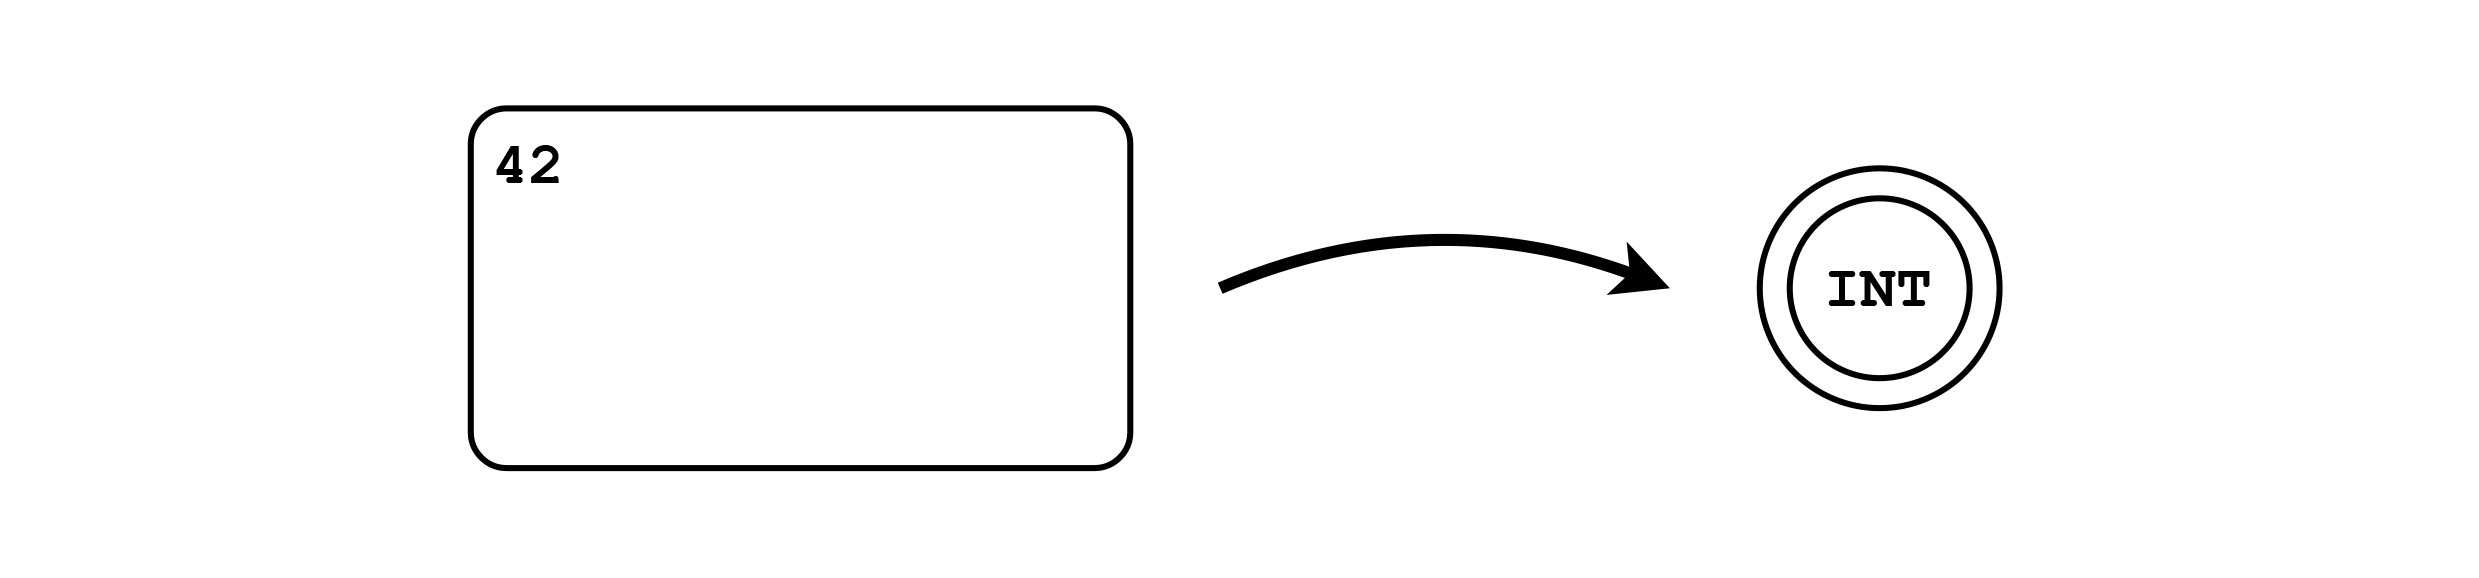
\includegraphics[scale=0.4]{imgs/msc-int.png}
	\caption{Budowanie grafu dla literału liczby całkowitej}
	%\label{fig:graph-int}
\end{figure}

Tak samo jest z literałami liczbami wymiernych, zmiennopozycyjnych, zespolonych oraz wartości \texttt{true}, \texttt{false} oraz \texttt{nil}.

Podobnie sytuacja ma się w przypadku literałów tekstowych (wierzchołek rodzaju \texttt{str}) oraz symboli (wierzchołek rodzaju \texttt{sym}). Drobna różnica jest taka, że tekst może być z interpolacją (np. \texttt{``foo\#\{somevariable\}bar''}), a w takim przypadku najpierw rekurencyjnie przetwarzamy wszystkie interpolowane (?) wyrażenia, ponieważ typ wyrażeń interpolowanych też może być potrzebny programiście. Jednakże, funkcja wnioskująca przypisuje wierzchołkowi rodzaju \texttt{str} zawsze typ \texttt{Nominal(String)} niezależnie od krawędzi wejściowych. Analogicznie jest w przypadku symboli.

\subsection{Literały tablic}

Pierwszym ciekawym przypadkiem jest literał tablicy, np. \texttt{[42, ``string'']}. Dla takiego AST, najpierw budujemy wierzchołki dla wszystkich poddrzew - w tym przykładzie dostaniemy dwa wierzchołki, odpowiednio rodzaju \texttt{int} oraz \texttt{str}. Następnie dodajemy wierzchołek rodzaju \texttt{array}, który będzie wynikiem przetwarzania tego AST, oraz dodamy krawędzie z wierzchołków \texttt{int} i \texttt{str} do wierzchołka \texttt{array}.

\begin{figure}[htb]
	\centering
	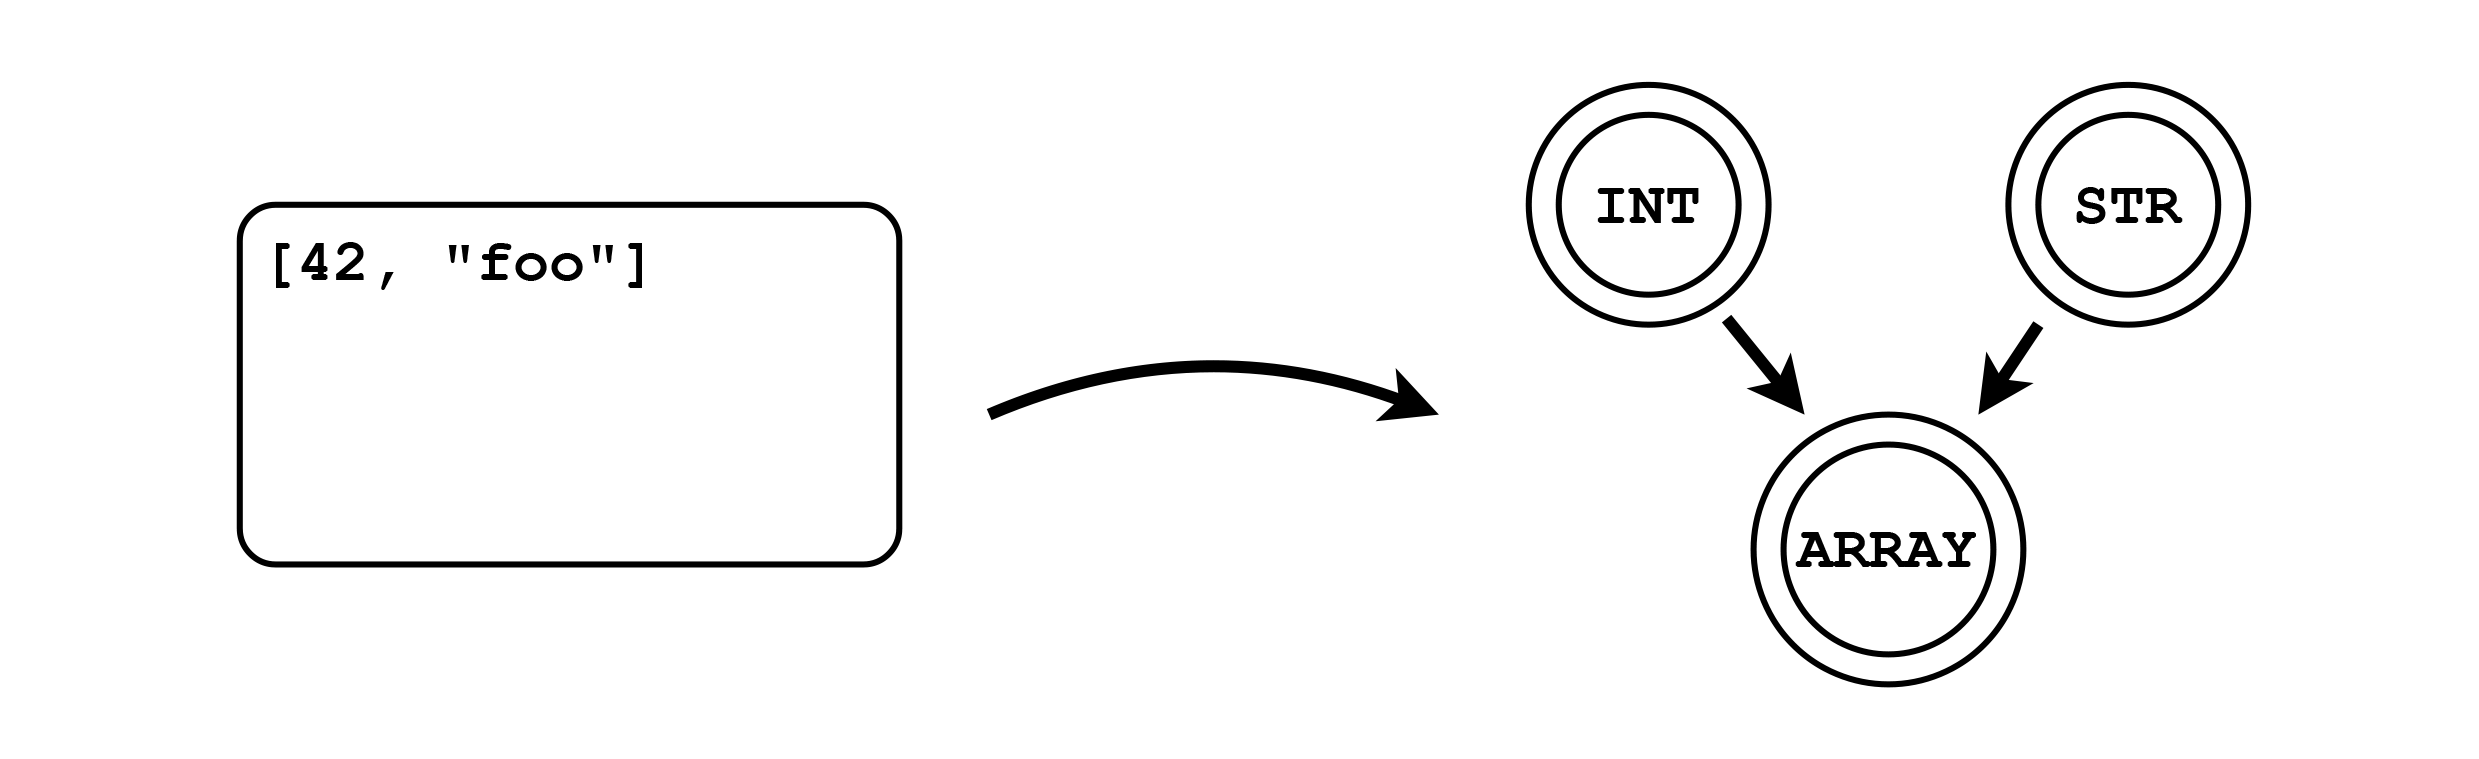
\includegraphics[scale=0.4]{imgs/msc-array.png}
	\caption{Budowanie grafu dla literału tablicy}
\end{figure}

Funkcja wnioskująca typ dla wierzchołka rodzaju \texttt{array} zawsze patrzy na typy wszystkich wierzchołków krawędzi wejściowych, tworzy z nich jeden typ Union -- w naszym przykładzie \texttt{Union(Integer or String)} oraz finalnie przypisuje temu wierzchołkowi typ parametryzowany \texttt{Generic(Array)<Union(Integer or String)>}.

\subsection{Słowniki}

W słownikach zarówno klucze i wartości mogą być różnego typu. Literał budowania słownika może również w sobie zawierać klucze (i oczywiście wartości), które nie są literałami. Przetwarzając literał słownika, budujemy trzy wierzchołki: \texttt{hash}, \texttt{hash\_keys} i \texttt{hash\_values}. Następnie przetwarzamy wszystkie klucze, oraz dodajemy dla każdego klucza krawędź pomiędzy wierzchołkiem wyrażenia klucza, a wierzchołkiem \texttt{hash\_keys}. Podobnie przetwarzamy wszystkie wartości i dodajemy krawędź pomiędzy wierzchołkami wartości, a wierzchołkiem \texttt{hash\_values}. Na końcu, dodajemy dwie krawędzie: pomiędzy \texttt{hash\_keys} oraz \texttt{hash} i \texttt{hash\_values} oraz \texttt{hash}.

Funkcja wnioskująca typ dla wierzchołka rodzajów \texttt{hash\_keys} oraz \texttt{hash\_values} działa grupująco - tj. zbiera wszystkie typy z wierzchołków z krawędzi wejściowych i łączy je w jeden typ \texttt{Union(...)}.
Funkcja typująca wierzchołek \texttt{hash} patrzy na rodzaje wierzchołków i buduje finalny typ \texttt{GenericType(Hash)<typ otrzymany z hash\_keys, typ otrzymany z hash\_values>}.

\subsection{Zmienne globalne}

W ogólności nie możemy wiedzieć w jakiej kolejności zostaną zmienne globalne, więc zakładamy, że w momencie referencji zmiennej globalnej jej wartość może pochodzić z dowolnego przypisania tej zmiennej w całym kodzie źródłowym. W tym celu, dla każdego identyfikatora (nie wystąpienia!) zmiennej globalnej tworzymy specjalny wierzchołek rodzaju \texttt{gvar\_definition} (\texttt{gv\_def} na rysunku). Za każdym razem gdy przetwarzamy przypisanie jakiejś wartości do danej zmiennej globalnej, tworzymy krawędź od tej wartości, do danego wierzchołka \texttt{gvar\_definition}. Odpowiednio, przetwarzając referencję zmiennej globalnej, tworzymy krawędź od \texttt{gvar\_definition} do tej wartości. W ten sposób, funkcja wnioskująca typy przekaże wszystkie możliwe przypisania danej zmiennej globalnej do wszystkich ich wystąpień w programie.

\begin{figure}[htb]
	\centering
	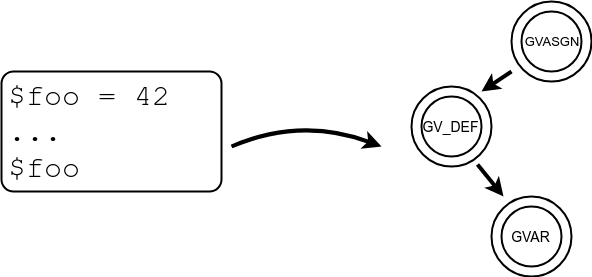
\includegraphics[scale=0.4]{imgs/msc-gvars.png}
	\caption{Budowanie grafu dla zmiennych globalnych}
\end{figure}

\subsection{Klasy i moduły}

Funkcja budująca graf, przyjmuje jako zależność instancję Bazy danych - na początku przetwarzania projektu pustą. W bazie przechowujemy wszystkie informacje, które pozwalają nam szybko odpowiadać na żądania, które wysyła do nas użytkownik. Dlatego też przechowujemy tam informacje np. o znalezionych podczas budowania grafu definicjach stałych i metod.

Podczas przechodzenia przez AST pliku, przetwarzając wierzchołek definicji klasy lub modułu, zapisujemy tę definicję w bazie. W Ruby klasa (i moduł) są wartościami, więc odrębnie zapisujemy definicję klasy (i informację np. o jej rodzicu), a oddzielnie fakt, że klasa ta została przypisana do pewnej stałej. Pozwala to na wspieranie otwartych klas, oraz w przyszłości (przyp: mogę w sobie w pracy magisterskiej mówić o 'przyszlosci'?) klas/modułów anonimowych.

Funkcja budująca graf jest funkcją rekurencyjną przekazującą sobie dwa argumenty: podgraf AST do przetworzenia, oraz kontekst. Kontekst przechowuje kilka informacji o aktualnym stanie budowania grafu. Po pierwsze, wie w jakim zagnieżdżeniu klas / modułów jesteśmy, oraz jeżeli aktualnie przetwarzamy definicję metody, to co to jest za metoda. W kontekście staramy się również w miarę możliwości śledzić czym jest aktualnie \texttt{self}. Ponadto, mamy słownik mapujący identyfikatory obecnych zmiennych lokalnych do ich możliwych definicji (w stylu klasycznej analizy statycznej \textit{Reaching Definitions}). Wreszcie, trzymamy w nim też krótką informację o aktualnie zadeklarowanej widzialności definiowanych metod (publiczne, prywatne lub chronione).

\subsection{Inne stałe}

Ponieważ zdefiniowane stałe mają domyślnie globalną widzialność oraz mogą być przypisywane ponownie, ich przypisywanie nie różni się bardzo od zwykłych zmiennych globalnych. Po pierwsze, odróżnia je to, że nie są prostym identyfikatorem (jak \texttt{\$foo}), ale złożonym z kilku, niekoniecznie statycznych (jeśli \texttt{x = Foo} to \texttt{x::Bar} jest poprawną referencją do \texttt{Foo::Bar}), więc wymagają specjalnych struktur danych w bazie, algorytmu rozwiązywania tych referencji i (przez to, że referencje mogą być dynamiczne) niekoniecznie są zawsze obliczalne w statycznej analizie.

Jest to też pierwsze miejsce, w którym stosujemy heurystyki bazujące na popularnych idiomach w Ruby. Przykładowo, w wyrażeniu \texttt{NetworkError = Class.new(StandardError)} najpierw tworzymy klasę anonimową dziedziczącą po klasie \texttt{StandardError}, a następnie przypisujemy ją do stałej \texttt{NetworkError}. Normalnie, nie wiedzielibyśmy o tym, że \texttt{NetworkError} jest klasą (bo nie śledzimy wartości), ale stosujemy heurystykę szukającą wyrażenia wg wzoru \texttt{X = Class.new(Y)}. Jeżeli heurystyka znalazła takie wyrażenie, to postępujemy z nim podobnie jak z definicją klasy. W przeciwnym przypadku, jak z definicją zwykłej stałej.

\subsection{Metody}

Podobnie jak jest to ze stałymi, podczas budowania grafu zapisujemy w Bazie znalezione definicje metod. Dokładniej, zapisujemy nazwę, identyfikator definicji klasy/modułu wewnątrz której została metoda zdefiniowana, drzewo argumentów formalnych (w Ruby argumenty formalne przez dekonstruktory mają postać drzewa), widoczność, oraz lokalizację w pliku. Zapisujemy też w bazie wierzchołki odpowiadające argumentom formalnym i wartości zwracanej przez metodę.

\subsection{Zmienne lokalne}

Tak jak zostało to wspomniane, wierzchołki o przypisaniach zmiennych lokalnych są przechowywane w kontekście w postaci podobnej do klasycznej statycznej analizy \textit{Reaching Definitions}, więc są dość dokładne. Podczas przechodzenia przez AST, w kontekście przekazujemy słownik mapujący identyfikatory zmiennych lokalnych w aktualnym \textit{lexical scope} na możliwe przypisania danej zmiennej lokalnej, a dokładniej -- wierzchołki tych przypisań.

\subsection{Dziedziczenie}

Ruby wspiera wiele rodzajów dziedziczenia, ale poszczególne konstrukty nie są od siebie istotnie różne. Jednak ponieważ to po czym dziedziczymy, składniowo, nie musi być identyfikatorem, ale może być dowolnym wyrażeniem (więc poprawne są konstrukty typu \texttt{class Foo < \$x} czy \texttt{class Foo < self}), znowu niemożliwa jest w pełni poprawna analiza. Aktualnie ograniczamy się tylko do obsługiwania sytuacji gdy to po czym dziedziczymy jest poprawnym identyfikatorem stałej, w przeciwnym wypadku ignorujemy to wyrażenie. W przyszłości łatwo można by wprowadzić heurystykę pozwalającą np. na dziedziczenie po strukturach (\texttt{class Foo < Struct.new(:field)}), ponieważ jest kilka takich idiomatycznych przypadków w których dziedziczymy po wyrażeniach nie będących identyfikatorami.

\subsection{Zmienne instancji}

Skoro Ruby jest językiem obiektowym, nie może zabraknąć zmiennych instancji. Aktualnie traktujemy je w podobny sposób jak zmienne globalne - nie próbujemy śledzić dokładnego flow, tylko zbieramy wszystkie możliwe przypisania zmiennych instancji, wszystkie możliwe użycia, i je łączymy ze sobą przez wierzchołek pośredni \texttt{ivar\_definition}. Aktualnie ignorujemy fakt, że zmienna \texttt{@x} w klasie \texttt{Foo} i \texttt{Bar} jest tą samą zmienną, jeśli \texttt{Bar} jest rodzicem \texttt{Foo}, ale łatwo rozszerzyć kod o tę funkcjonalność (przyp: może to jeszcze zrobię w sumie, bo szkoda tego tłumaczenia).

\subsection{Eigenclass}

Ruby, będąc językiem w pełni obiektowym, nie ma mechanizmu metod statycznych znanego np. z C++, ale ma podobnie działające tzw. metody klasowe. Klasy są obiektem, a jeżeli coś jest obiektem (instancją) to musi mieć również swoją klasę. Naturalnym wydawałoby się, że klasa jest instancją klasy \texttt{Class}, ale w Ruby mamy dodatkowy element -- każda definicja klasy tworzy dla tej klasy również \texttt{eigenclass}. Właściwym łańcuchem dziedziczenia jest więc \texttt{Foo < eigenclass Foo < Class}.

Otwierając definicję klasy (ale gdy ciągle nie jesteśmy wewnątrz definicji metody), \texttt{self} jest właśnie instancją tej \textit{eigenclass}. W definicji klasy możemy wtedy korzystać ze składni \texttt{def self.foo} aby zdefiniować metodę na \textit{eigenclass} lub \texttt{class << self} aby otworzyć definicję \textit{eigenclass}. W ten sposób zdefiniowane metody zachowują się jak metody statyczne, tj. można je wywołać przez składnię \texttt{PewnaKlasa.foo(...)}.

Składnie te są reprezentowane przez konkretne wierzchołki, ale w miejscu \texttt{self} może być dowolne wyrażenie -- możemy więc napisać np. \texttt{def Foo.bar} i zdefiniować metodę na \textit{eigenclass} klasy \texttt{Foo} będąc wewnątrz kompletnie innej metody.
Jednakże prawie zawsze jest to \texttt{self}, więc obsługujemy tylko tę składnię.
Obsługa definicji metody wewnątrz \textit{eigenclass} (\texttt{def self.foo; ...; end}) lub definicji \textit{eigenclass} (\texttt{class << self; ...; end}) są bardzo podobne do zwykłej definicji metody lub klasy, z tą różnicą, że zamiast zdefiniować metodę na klasie, najpierw pobieramy z bazy \textit{eigenclass}, a dopiero potem dodajemy definicję.
Jeśli \textit{eigenclass} nie ma, to dodajemy pustą definicję klasy jako tę właśnie \textit{eigenclass}.


\subsection{attr reader, private}

Są wbudowane w Ruby metody \textit{klasowe}, które definiują inne metody, więc są już de facto metaprogramowaniem.
W bibliotece standardowej Rubiego najpopularniejsze to \texttt{attr\_reader} i \texttt{attr\_writer}.
\texttt{attr\_reader(:foo)} definiuje metodę odczytującą zmienną instancji, o takiej samej nazwie, jest więc odpowiednikiem kodu \texttt{def foo; @foo; end}. Oczywiście, \texttt{attr\_reader} przyjmuje dowolną liczbę argumentów, więc szybko można za jego pomocą zdefiniować wiele takich funkcji.

Tutaj funkcja budująca ucieka się do heurystyki wykrywającej użycie funkcji o nazwie \texttt{attr\_reader} i zamiast uznawać to wywołanie za zwykłe wywołanie metody, definiuje odpowiednią metodę dla każdego argumentu. Dodatkowo, ustawia lokalizację występowania definicji tak zdefiniowanej metody na linijkę z \texttt{attr\_reader}, więc programista, który użyje skoku do definicji łatwo dowie się, że metoda ta jest definiowana za pomocą \texttt{attr\_reader}. Bardzo podobnie jest z metodą \texttt{attr\_writer}, która definiuje przypisanie do zmiennej instancji (tzw. \textit{setter}).

\subsection{Widzialność metod}

W większości języków obiektowych, \texttt{private}, \texttt{public} i \texttt{protected} są słowami kluczowymi (a przez to - posiadają własne AST), w Ruby jednakże są to zwykłe wywołania metod klasowych. Z tego powodu, znowu korzystamy z heurystyk. W tym wypadku jednak takie heurystyki są mniej akceptowalne, ponieważ te nazwy mogą prawdopodobnie pojawić się w produkcyjnych programach -- natknąłem się na ten problem osobiście (przyp: nie wiem czy powinienem pisać takie rzeczy, w pierwszej osobie). Jednak z braku lepszego rozwiązania, stosujemy tutaj również tylko prostą heurystykę po nazwie metody. W tym wypadku, analizujemy argumenty jakie otrzymuje wywołanie metody \texttt{private} i wysyłamy do bazy żądanie zmiany widzialności metod o podanych jako argumenty nazwach, w definicji klasy którą aktualnie przetwarzamy (informację o aktualnie przetwarzanej definicji klasy trzymamy w kontekście).


\subsection{Wywołania metod}

Pomimo tego, że jest to prawdopodobnie najważniejszy AST, jego analiza podczas budowania grafu nie jest bardzo skomplikowana. Funkcja budująca przetwarza rekurencyjnie wyrażenie na którym wywoływana jest metoda oraz przekazywane argumenty. Następnie tworzy dodatkowy wierzchołek na wynik tej metody. Wreszcie, wszystkie te wierzchołki łączy w rekord i wrzuca do kolejki wywołań. Kolejka ta będzie używana dopiero podczas typowania.

\subsection{Wywołania super}

Wywołania \texttt{super} dzielą się na dwa rodzaje (i są to dwa różne wierzchołki AST). Pierwszy to zwykłe wywołanie \texttt{super(args)} znane z innych języków programowania, wywołujące odpowiadającą metodę z definicji rodzica i przekazującą podane do \texttt{super} argumenty. Analiza tego wywołania jest bardzo podobna do zwykłego wywołania metody poza tym, że do rekordu wywołania dopisujemy jeszcze identyfikator aktualnie przetwarzanej metody, aby łatwo znaleźć rodzica i odpowiadającą w nim metodę.

Drugi rodzaj wywołania jest bezargumentowy, tj. \texttt{super}. W takim wypadku, wszystkie argumenty przekazane do tej metody są przez interpreter podane do tego bezargumentowego wywołania \texttt{super}, tj. metoda rodzica zostaje wywołana dokładnie z takimi samymi argumentami. W takim wypadku, jedyne co robimy to zapisujemy w bazie wierzchołek odpowiadający wywołaniu bezargumentowego \texttt{super}.


\subsection{Bloki i lambdy}

Jak w większości współczesnych języków programowania, w Ruby również funkcje są \textit{first class citizens}, a więc są wartościami, które mogą być przypisywane do zmiennych i przekazywane jako argumenty. W Ruby są obecne też bloki, które są niczym innym jak przekazywaną do wywołania metody funkcją, którą można wywoływać wewnątrz metody za pomocą specjalnej składni \texttt{yield}. Każde użycie składni \texttt{yield} wewnątrz metody wywołuje tę funkcję i przekazuje do niej argumenty (jeśli zostały jakieś przekazane do \texttt{yield}).

Analizując słowo kluczowe \texttt{yield}, tworzymy specjalny rekord składający się z przekazanych argumentów i specjalnego wierzchołka na wynik - bardzo podobnie jak w przypadku wywołania metody. Dodajemy ten rekord do specjalnej listy użyć \texttt{yield} połączonej z definicją aktualnie przetwarzanej metody.

Analizując blok, podejmujemy działania podobne, jak przy definiowaniu zwykłej metody, tj. analizujemy argumenty, przygotowujemy wierzchołki na argumenty formalne, wierzchołek na wynik bloku i wszystko łączymy w rekord. Ruby nie posiada specjalnego słowa kluczowego na zbudowanie funkcji anonimowej, jest to po prostu blok przekazany do funkcji o nazwie \texttt{lambda}. Prosta heurystyka znowu pozwala rozróżnić przypadki, kiedy po prostu budujemy funkcję anonimową, a kiedy przekazujemy blok do wywołania metody. W tym pierwszym przypadku, zapisujemy identyfikator (automatycznie wygenerowany, na potrzeby analizy) tej funkcji w wierzchołku, a w drugim -- zapisujemy ten identyfikator przy wywołaniu metody.

% foo(&x)
% foo(&:x)

\subsection{Biblioteka standardowa}

Ruby jest językiem interpretowanym, więc definicje podstawowych klas i metod są bezpośrednio w interpreterze. Interpreter jest napisany w C, więc tych definicji nie ma napisanych w Ruby. Aby nasza analiza była praktyczna, definicje biblioteki standardowej powinny być w pewien sposób obsłużone.

Metody w bibliotece standardowej możemy podzielić na dwie grupy. W większości metod, jedyne co nas interesuje to zwracany typ -- wyobraźmy sobie metody typu \texttt{File.read(filepath)}. Wystarczające jest jeżeli o tej metodzie zapiszemy, że zawsze zwraca typ \texttt{NominalType(String)}. W taki sposób możemy sobie poradzić z większością metod.

Cięższym przypadkiem są metody przetwarzania danych, takie jak \texttt{map} lub \texttt{filter} w klasie \texttt{Array}. Tablica jest typem parametryzowanym (np. \texttt{Generic(Array)<Integer>}), więc nie ma tutaj stałego typu który moglibyśmy uniwersalnie zwracać. Drugą opcją byłoby dodanie odpowiednich wierzchołków i krawędzi odpowiadających temu, jak dana metoda działa i traktowanie jej dokładnie tak samo jak zwykłe metody podczas typowania (jedyną różnicą byłoby więc to, że graf dla definicji tej metody byłby napisany przez autora analizy, a nie automatycznie na podstawie AST). Jednak podczas typowania, łączymy każde użycie metody z tą samą definicją formalną. Oznaczałoby to, że jeżeli w dwóch różnych miejscach kodu wywołujemy metodę \texttt{map}, raz na obiekcie typu \texttt{Generic(Array)<Integer>}, a raz na \texttt{Generic(Array)<String>}, to wywnioskowanym zwracanym typem dla obu tych wywołań byłby \texttt{Generic(Array)<Integer or String>}. A ponieważ w praktyce wywołujamy \texttt{map} na listach wielu różnych obiektów, taki zwracany typ byłby bardzo długi i bezużyteczny.

Trzecią opcją byłoby zapisanie przez autora analizy tylko wzoru jak wygląda graf dla tej definicji metody, ale tworzenie świeżych wierzchołków i krawędzi tego grafu w każdym miejscu, w którym ta metoda jest wywoływana. Jest to rozwiązanie przyjęte w tej pracy. Oczywistą wadą jest większy rozmiar grafu, ale rozwiązanie to sprawdza się w praktycznych zastosowaniach.

\subsection{self}

\texttt{self} jest konstrukcją języków zorientowanych obiektowo, która sprawia problemy przy analizie statycznej.
Jest tak ponieważ \texttt{self} jest jednocześnie bardzo często używany (w szczególności właściwie wszystkie wywołania metod prywatnych to wywołania na wyrażeniu \texttt{self}) oraz jego dokładny typ jest trudny do określenia. Nasza analiza korzysta z bardzo uproszczonego założenia, że \texttt{self} jest zawsze typem odpowiadającym definicji klasy, w której jest użyte. W przyszłości jednak można by było spróbować z założeniem, że \texttt{self} jest typu odpowiadającym danej definicji klasy lub jednym z jej podklas. Z jednej strony, takie rozwiązanie byłoby bardziej bezpieczną analizą. Z drugiej strony, w każdym projekcie są klasy podstawowe, po których dziedziczy wiele innych definicji klas. W takich przypadkach bezpieczniejsze podejście mogłoby się okazać niepraktyczne, ponieważ \texttt{self} byłby typowany jako unia np. 100 różnych klas. (przyp: chyba te ostatnie dwa zdania trochę nieskładnie)

\subsection{Wyjątki}

Obsługa wyjątków nie jest skomplikowana i główną trudnością jest odpowiednie obsłużenie \textit{lexical scope} dla zmiennych lokalnych. Jedyną rzeczą wartą wspomnienia jest fakt, że \texttt{raise SomeError} jest pierwszym przykładem wyrażenia, któremu celowo przypisujemy podczas typowania typ \texttt{Bottom} (tj. brak typu), ponieważ nie zwraca to wyrażenie żadnej wartości.

\subsection{Pętle}

Pętle i słowa kluczowe z nimi związane (\texttt{break}, \texttt{next} itp.) również nie są zbyt interesujące. Po pierwsze dlatego, że z reguły wyrażenia związane z pętlami zwracają \texttt{nil} lub nic (tj. są typu \texttt{Bottom}), więc jedyne na co trzeba uważać to znowu, poprawne obsłużenie \textit{lexical scope} zmiennych lokalnych. Po drugie dlatego, że pętle w ruby są używane bardzo rzadko i iteracje w idiomatycznym Ruby wyraża się za pomocą funkcyjnych \texttt{map}, \texttt{filter}, \texttt{each} i innych.

\subsection{Return}

Ruby posiada znane z innych języków programowania słowo kluczowe \texttt{return}, kończące wykonywanie funkcji i zwrócenie wartości jako wynik funkcji. Aby to wspierać, pobieramy z kontekstu wierzchołki aktualnie przetwarzanej metody, a wśród nich wierzchołek rodzaju \texttt{call\_result}. Jedyne co musimy zrobić to dodać krawędź pomiędzy wierzchołkiem wyrażenia przekazanego w \texttt{return}, a wierzchołkiem \texttt{call\_result} pobranym wcześniej z kontekstu.


\section{Wnioskowanie typu}

\subsection{Typy}

Mamy następujące typy:

\begin{itemize}
 \item \texttt{Bottom} - typ oznaczający brak typu, używany kiedy typ wierzchołka jest jeszcze nie znany lub typu nie posiada (np. słowa kluczowe \texttt{raise} lub \texttt{break})
 \item \texttt{NominalType(Foo)} -- podstawowy typ, oznacza że wyrażenie jest instancją klasy Foo.
 \item \texttt{ClassType(Foo)} -- typ oznaczający że wyrażenie jest klasą \texttt{Foo}. Innymi słowy, jest instancją klasy \texttt{Class} lub instancją \textit{eigenclass} klasy \texttt{Foo}, ale tak dokładna informacja jest oczywiście przydatniejsza niż samo \texttt{NominalType(Class)}, dlatego mamy oddzielny typ na ten specjalny przypadek.
 \item \texttt{GenericType(Foo)<typ1, typ2, ...>} -- typ oznaczający jeden z typów generycznych. Opisane w pracy są dwa: \texttt{Array} posiadający jeden parametr, oraz \texttt{Hash} posiadający dwa parametry (typ kluczy i typ wartości). Parametry są typami. Można sobie łatwo wyobrazić rozszerzenie na inne klasy z biblioteki standardowej, takie jak \texttt{Set} lub \texttt{Range}.
 \item \texttt{UnionType(typ1, typ2, ...)} -- typ oznaczającą dowolny z wymienionych typów. Większość rodzajów wierzchołków w funkcji typującej jedyne co robi to bierze typy z wszystkich wierzchołków wejściowych i tworzy z nich jeden \texttt{UnionType}.
 \item \texttt{MainType} -- typ szczególny, mało istotny w typowaniu. Definicje metod, które są zdefiniowane nie w definicji klasy, są zdefiniowane na specjalnym obiekcie \texttt{main}.
\end{itemize}


\subsection{Funkcja wnioskująca typy}

Kiedy graf jest gotowy, przekazujemy go do funkcji wnioskującej typy wszystkich wierzchołków. Funkcja ta jest podzielona na kilka etapów.
Do kolejki z wierzchołkami są na początku dodawane wszystkie wierzchołki, a typ wszystkich jest ustawiany na \texttt{Bottom}.
Następnie przetwarzamy każdy wierzchołek (nazwijmy go \texttt{X}) z kolejki.
Jeżeli po inferencji typu, typ wierzchołka \texttt{X} się zmienił, patrzymy na wszystkie krawędzie wychodzące z \texttt{X} i dodajemy docelowe wierzchołki tych krawędzi do kolejki, jeśli ich tam jeszcze nie ma.
Gdy przetworzymy wszystkie wierzchołki, przechodzimy do przetwarzania wywołań metod.
Wywołanie metody przetwarzamy tylko, jeśli wszystkie jej argumenty oraz obiekt na którym wywoływana jest metoda, są ukonkretnione (tj. żaden z nich nie jest typu \texttt{Bottom}).
Następnie, w zależności od obliczonego typu wyrażenia na którym jest wywoływana metoda, oraz jej nazwy, zachodzi kilka heurystyk opisanych w następnych częściach.

Schemat we wszystkich jest podobny i polega na znalezieniu w bazie definicji metody, która została wywołana, a następnie połączeniu wierzchołków argumentów wywołania (przyp: jest jakaś lepsza polska nazwa na tzw. actual arguments?) z argumentami formalnymi oraz wierzchołka wyniku metody z wierzchołkiem wyniku wywołania.
Dzięki temu że wszystkie argumenty są zdefiniowane, możemy tutaj przeprowadzić kilka dodatkowych heurystyk.
Są obecne specjalne mechanizmy pilnujące, że daną definicję metody przypiszemy do danego wywołania tylko raz (bo wywołania mogą być przetwarzane więcej niż raz).
Następnie, jeśli w efekcie przetwarzania metod zostały dodane jakieś wierzchołki do kolejki, to wracamy do etapu przetwarzania wierzchołków.
Jeżeli żadne nie zostały dodane, to przetwarzamy znowu wywołania metod, tym razem obsługując wywołanie nawet wtedy, jeśli któryś z argumentów nie jest zdefiniowany.

\subsection{Heurystyki obsługi wywołań}

Na początku sprawdzamy czy wywołanie nie pasuje do jednej z heurystyk opisanych poniżej. W przeciwnym przypadku zakładamy że to jest zwykłe wywołanie, które w szczególe zostanie omówione w następnej sekcji.

Po pierwsze, wywołanie może wyglądać jak wywołanie konstruktora, tj. jest wywoływana metoda \texttt{new} na typie reprezentującym klasę. Ten przypadek jest prawie taki sam jak obsłużenie zwykłego wywołania metody z tą różnicą, że zamiast zwrócić wynik konstruktora, zwracamy typ instancji zamiast typu klasowego na którym konstruktor był wywołany, tj. jeżeli konstruktor był wywołany na wierzchołku typu \texttt{ClassType(Foo)} to zwracamy typ \texttt{NominalType(Foo)}.

Drugim przypadkiem jest kiedy obiekt na którym wywołujemy metodę jest typu \texttt{ProcType}, a nazwa metody to \texttt{call}. Oznacza to wywołanie funkcji anonimowej. W \texttt{ProcType} trzymamy identyfikator funkcji anonimowej, wystarczy go więc tylko pobrać i wyciągnąć z bazy definicję funkcji -- reszta procedury jest taka jak w przypadku zwykłego wywołania metody.

Trzeci przypadek to metoda klasowa. Uznajemy wywołanie za wywołanie metody klasowej, jeśli obiekt na którym wywołujemy metodę jest pewnego typu klasowego, tj. \texttt{ClassType}. W tym przypadku jedyną różnicą od zwykłego wywołania jest zapytanie do bazy danych, które szuka metod zdefiniowanych na eigenclass, a nie w definicji klasy.

Tak jak zostało wspomniane wyżej, jeżeli żaden z tych przypadków nie zachodzi, uznajemy wywołanie za klasyczne wywołanie metody na instancji pewnego obiektu. Szukamy w takim wypadku metody o odpowiadającej do wywołania nazwie, która została zdefiniowana w klasie obiektu na którym metoda jest wywoływana.

\subsection{Obsługa wywołania}

Po powyższych heurystykach możemy założyć, że mamy już znalezioną definicję metody, do której chcemy podłączyć wywołanie. Definicja, niezależnie od tego czy była to klasyczna definicja metody czy definicja funkcji anonimowej, ma obowiązkowo kilka właściwości: drzewo argumentów formalnych, wierzchołek wyniku definicji, listę użyć bezargumentowego super, listę użyć słowa kluczowego \texttt{yield} (tj. wywołań bloków) oraz być może wierzchołek wywoływacza (wierzchołek wywoływacza jest specjalnym mechanizmem, opisanym dokładniej w sekcji poświęconej wywołaniom polimorficznym).

Najpierw następuje dodanie krawędzi między wierzchołkiem obiektu, na którym jest wywoływana metoda, oraz specjalnego wierzchołka rodzaju \texttt{caller} dla tej definicji metody, o ile on istnieje.

Najważniejsza część to wspomniane już połączenie wierzchołków argumentów wywołania z wierzchołkami argumentów formalnych, oraz wierzchołka wyniku metody z wierzchołkiem wyniku wywołania. Są dwa powody, które utrudniają zrobienie poprawnego dopasowania argumentów wywołania i argumentów formalnych.

Pierwszym jest tzw. \textit{splat argument}. Zarówno w argumentach wywołania jak i argumentach formalnych, możemy użyć składni \textit{splat}, która w przypadku argumentów wywołania spłaszcza przekazaną listę jako listę argumentów, a w przypadku argumentów formalnych buduje tablicę z przekazanych argumentów. Jest to mechanizm znany z wielu języków pozwalający na definiowanie i wywoływanie funkcji o zmiennej liczbie argumentów. 

Drugi to \textit{named arguments} czyli argumenty, które w wywołaniu muszą być przekazane razem z nazwą argumentu formalnego, ale dzięki temu mogą być przekazane w dowolnej kolejności. Niestety, jest to tylko pewna sztuczka głównie po stronie parsera. Mechanizm \textit{named arguments} w Ruby polega na tym, że jeżeli ostatni przekazywany argument jest słownikiem, to jest traktowany jako słownik zawierający przekazywane \textit{named arguments}. Z tego powodu, przekazywane argumenty wcale nie muszą być przekazywane explicit, ale mogą być przekazane np. przez zwykłą zmienną, która jest słownikiem. Dlatego też aby poprawnie dopasować przekazane \textit{named arguments} do tych w definicji wywołania, musielibyśmy śledzić dokładne mapowanie typów w każdym słowniku.

Trzecim etapem jest połączenie przekazanych argumentów do metody z klasy nadrzędnej oraz wyników tej metody z wszystkimi wywołaniami bezargumentowego \texttt{super}.

Kolejnym krokiem jest obsługa bloku. Blok mamy przypisany do wywołania, z reguły w postaci albo w postaci wierzchołka z identyfikatorem funkcji anonimowej (tj. przekazany blok był znany już przy budowaniu grafu), albo wierzchołka grafu, który został otypowany na \texttt{ProcType} i zawiera w sobie identyfikator funkcji anonimowej. Następuje więc przejście po wszystkich użyciach słowa kluczowego \texttt{yield} w tej metodzie i połączeniu przekazanych do \texttt{yield} argumentów z argumentami formalnymi znalezionej funkcji anonimowej oraz wierzchołka wyniku funkcji anonimowej z wierzchołkiem wyniky \texttt{yield}. Jest to procedura identyczna do opisanego wyżej łączenia argumentów wywołania z argumentami formalnymi.

Na końcu, następuje połączenie wierzchołka wyniku metody oraz wierzchołka wyniku wywołania.


\subsection{Wywołania funkcji polimorficznych}

Jak już zostało wspomniane, definicja metody w Bazie ma w sobie kilka wierzchołków, które są istotne z punktu widzenia analizy, takie jak wierzchołek wyniku metody, wierzchołki argumentów i inne związane z blokami i wywołaniami bezargumentowego \texttt{super}. Te wierzchołki mogą zostać przechowywane na dwa sposoby. Pierwszy z nich to po prostu dokładnie te wierzchołki, które są obecne w grafie. Drugi sposób to przechowywanie szkicu podgrafu (tj. wierzchołki i krawędzie, które nie należą do grafu -- są tylko wzorem), z którego przy okazji przetwarzania każdego wywołania są tworzone świeże wierzchołki.

Świeże wierzchołki dla każdego wywołania oznaczają też, że możemy skorzystać z typu wyrażenia na którym metoda została wywołana. Dlatego też, jeżeli obsługujemy wywołanie metody której definicja korzysta z podgrafu, łączymy wierzchołek wyrażenia na którym została wywołana metoda z wierzchołkiem rodzaju \texttt{caller}. Dzięki temu możemy bez problemu zbudować podgrafy działające poprawnie dla takich metod polimorficznych jak \texttt{map} z \texttt{Array} lub po prostu funkcje, które zwracają obiekt na którym zostały wywołane (nie było to możliwe bez podgrafu), takie jak np. \texttt{freeze}.

\subsection{Inne wierzchołki specjalne}

Podejście z podgrafami pozwala też na obsługę niektórych metod w specjalny sposób, bez dużej ingerencji w funkcję typującą. Przykładem takiej metody jest metoda \texttt{class}, którą możemy wywołać na dowolnym obiekcie, a która zwraca klasę tego obiektu. Dzięki podgrafowi, definicja takiej metody to tylko dwie krawędzie, widoczne na rysunku. Specjalny wierzchołek \texttt{extract\_class} na podstawie typu wierzchołka z krawędzi wejściowej zwraca odpowiedni typ, który zwróciłaby metoda \texttt{class}. Na przykład, jeżeli typ wejściowy to \texttt{NominalType(Foo)}, to typem wyjściowym będzie \texttt{ClassType(Foo)}.


%\section{Future work}

%\subsection{More metaprogramming intelligence}
%\subsection{Bundler, gems and libraries}
%\subsection{YARD}
%\subsection{Rust implementation}
%\subsection{Caching}
%\subsection{Tracking effects, ex. exceptions}
%\subsection{Tracepoint}


%%%%% BIBLIOGRAFIA

%\begin{thebibliography}{1}
%\bibitem{example} \ldots\
% https://yehudakatz.com/2009/11/15/metaprogramming-in-ruby-its-all-about-the-self/
%\end{thebibliography}

\end{document}
